\chapter{Organização de elementos do trabalho acadêmico}
%Exemplo de epígrafe de início de capítulo:
\begin{epigrafe}
    % Seu texto recomenda-se em itálico e autor em negrito
    \textit{O Guia de Normalização diz que você pode utilizar, se quiser, epígrafes no início de cada uma das seções primárias (capítulos). Eis aqui o exemplo. O Guia diz que você pode, mas será se você deve? Eu vou ser honesto, acho um pouco esquisitinho.} \textbf{Leonardo Garcez Dalenogari Alba}
\end{epigrafe}

%Falar as observações contidas no Guia
O Guia de normalização, com base na NBR 14724, estabelece um conjunto de elementos, opcionais\index{Elementos opcionais} e obrigatórios, que podem constar em um trabalho acadêmico. A organização desses elementos, divididos em elementos pré-textuais, textuais e pós-textuais, pode ser observada na Figura \ref{figura:elementos-guia}. E, neste capítulo, serão discutidas algumas observações sobre esses elementos, principalmente pré-textuais e pós-textuais, envolvendo suas particularidades no \LaTeX{}, neste modelo. Entretanto, a descrição, e melhor detalhamento, sobre o que deve estar contido em cada elemento estão no \citetitle{livro:iffar-guia-normalizacao-2022}, recomendando-se que faça-se a sua leitura.

\begin{figure}[H]
    \Centering\singlespacing
    \caption{Organização dos elementos do Trabalho Acadêmico-Científico}
    \label{figura:elementos-guia}
    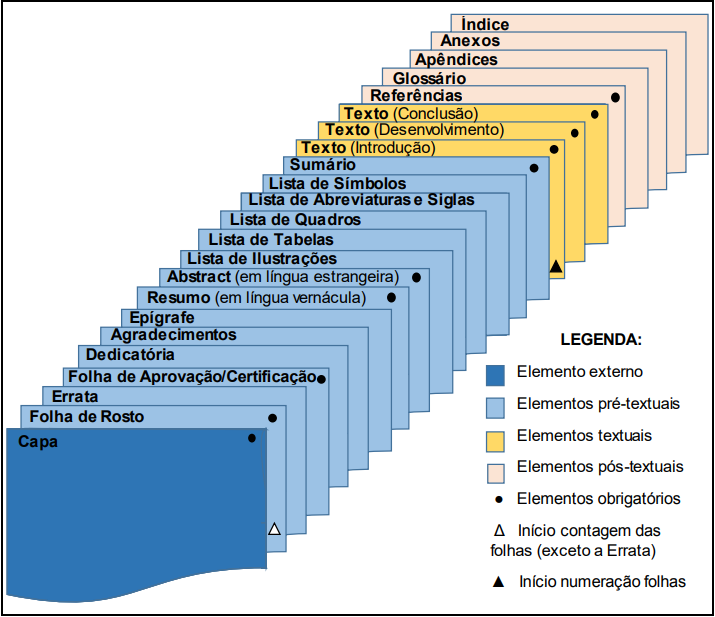
\includegraphics[width=10cm]{guia-elementos.png}
    
    \footnotesize
    Fonte: \textcite{livro:iffar-guia-normalizacao-2022}.
  \end{figure}

\section{Parte externa}
    \subsection{Capa (obrigatório)}
    Arquivo: \texttt{elementos/capa.tex}

    Não é computada na contagem das folhas.

    É configurado automaticamente pelo arquivo \texttt{elementos/DADOS.tex}. Selecione se o seu trabalho é TCC ou Tese e Dissertação e preencha os dados restantes com os valores necessários.

    O Guia de Normalização estabelece que a capa deve conter \blockcquote[p. 30]{livro:iffar-guia-normalizacao-2022}{nome da instituição (opcional), título do trabalho e nome do(a) autor(a)}, o mesmo estabelecido pela NBR 14724 \cite{livro:abnt-nbr:14724}, porém, nos seus exemplos visuais mostram-se dados adicionais\footnote{Eu implementei conforme o ilustrado, apesar de não saber sobre a definição de margens.}.

    \subsection{Lombada (opcional)}
    É utilizado para trabalhos impressos e, por isso, este modelo não abrange tal elemento.

\section{Elementos pré-textuais}
    Para o caso do uso da configuração \textbf{twoside}, para uso de verso e anverso das folhas: recomenda-se que seus elementos, com exceção da ficha catalográfica/de identificação, iniciem no anverso das folhas (parte da frente da folha, página ímpar). O modelo detecta e realiza a configuração para o início desses elementos\footnote{Porém, podem acontecer \textit{bugs}, pois o \texttt{cleardoublepage} é considerado um comando frágil pelo \LaTeX{}.}, você pode optar por desativar, comentando ou removendo os comandos \verb|\OnesideTwoside| no fim de cada elemento, apesar da utilização de pelo menos um \verb|\clearpage| ser recomendada\footnote{Mas também não acontece nenhum problema se não existir o comando}.

\subsection{Folha de rosto (obrigatório)}
    Arquivo: \texttt{elementos/folha-rosto.tex}

    Também configurado automaticamente pelo arquivo \texttt{elementos/DADOS.tex}. Caso a lógica criada para o preenchimento dos dados não funcione bem para a sua situação, não tenha receio em alterar diretamente o seu texto em seu arquivo.

    Para o caso do trabalho estar configurado como \textbf{twoside}, para a impressão no verso e anverso, configure, no final de seu arquivo, o uso do \verb|\clearpage|:
    \begin{alinea}
        \item se existir a ficha catalográfica\footnote{Que nem ao menos sei como que é realizado o processo, se o autor que adiciona no documento \LaTeX{} ou se o(a) bibliotecário(a) é responsável tanto por criar os dados quanto anexar depois no documento.}/identificação de obra, altere o comando \verb|\OnesideTwoside| e utilize \verb|\clearpage|, pois a ficha deve estar no verso;
        \item se ainda não possuir a ficha, seja qual for, deixe o comando \verb|\OnesideTwoside| decidir pelo \verb|\cleardoublepage|.
    \end{alinea}

\subsection{Ficha catalográfica ou ficha de identificação (obrigatório)}
    Arquivo: \texttt{elementos/ficha-catalografica.tex}

    A ficha catalográfica é elaborada pelos bibliotecários da instituição e a ficha de identificação é produzida pelos autores dos trabalhos, \blockcquote[p. 15]{livro:iffar-guia-normalizacao-2022}{partir de um sistema gerador que a instituição utilize}\footnote{Não tenho ideia alguma sobre esse sistema.}.

    Obrigatoriamente deve estar contida no verso da folha de rosto\footnote{Até mesmo utilizando \textbf{oneside}? Se for, acho que será necessário criar uma lógica diferente, pois assim não sei como que fica a contagem de páginas para este elemento.}.
    
\subsection{Errata (opcional)}
    Ocorre após a impressão do trabalho e, por isso, o modelo não abrange tal elemento. Se necessário, pode-se utilizar outra ferramenta de texto para gerar a errata, visto que só deve ser necessário manter a mesma fonte utilizada no trabalho.
    
\subsection{Folha de aprovação e/ou folha de certificação (obrigatório)}
    Arquivo: \texttt{elementos/folha-aprovacao.tex}

    Configurada automaticamente pelo arquivo \texttt{elementos/DADOS.tex}: para TCC é utilizada a folha de aprovação; e, para o caso de Tese ou Dissertação, utiliza-se a folha de certificação. Adicione seus dados e, se a lógica criada para o preenchimento dos dados não funcionar para o seu caso, não tenha receio de alterar manualmente o texto em seu arquivo.
    
\subsection{Dedicatória (opcional)}
    Arquivo: \texttt{elementos/dedicatoria.tex}

    Não possui título e a \blockcquote[p. 32]{livro:iffar-guia-normalizacao-2022}{a autoria de terceiros deve ser citada, e também deve constar nas Referências)}.

    Em \texttt{main.tex}, comente a linha \verb|\vspace*{\fill}

% Tamanho total da página: 21cm
% Margem esquerda: 3cm
% Margem direita: 2cm
% Recuo necessário: 4cm
% Espaço restante: 12cm
\hspace{\fill}
\begin{minipage}{12cm}
    \setlength{\parindent}{1.25cm}
    
    Este trabalho é dedicado [especificar o texto da dedicatória, escrito pelo(a) autor(a), registrando a quem dedica o Trabalho Acadêmico-Científico realizado ou prestando uma homenagem a alguém que considere importante no transcorrer do seu processo formativo (pessoal e/ou acadêmico-profissional), ainda que essa pessoa não tenha contribuído diretamente para os resultados obtidos no trabalho].
\end{minipage}

% Recomendação do Guia de Normalização de iniciar cada elemento pré-textual e textual no anverso da página
\OnesideTwoside{\clearpage}{\cleardoublepage}
| para não adicionar o elemento.

\subsection{Agradecimentos (opcional)}
    Arquivo: \texttt{elementos/agradecimentos.tex}

    \blockcquote[p.32]{livro:iffar-guia-normalizacao-2022}{Pode se constituir de um texto mais extenso, em que são mencionadas as contribuições relevantes para os resultados apresentados no trabalho.

    Sugere-se incluir a agência financiadora, indicando-se a fonte de
    financiamento que viabilizou a realização do estudo.}

    Em \texttt{main.tex}, comente a linha \verb|\chapter*{Agradecimentos}
\thispagestyle{empty}

\lipsum[2]| para não adicionar o elemento.

\subsection{Epígrafe (opcional)}
    Arquivo: \texttt{elementos/epigrafe.tex}

    Além de utilizar como elemento pré-textual, a epígrafe também pode ser utilizada para iniciar as seções primárias (capítulos) do seu trabalho, porém, é algo opcional. Para se criar uma epígrafe, utiliza-se de seu respectivo ambiente criado para este modelo, através do comando \verb|\begin{epigrafe}|.

    Nas epígrafes é recomendado o destaque em itálico para a citação e de negrito para a autoria dessa citação, que deve seguir o padrão para referenciamento, como sobrenome em caixa alta, ano e página envoltos entre parênteses, de acordo com o exemplo em \textcite[figura 14, p. 39]{livro:iffar-guia-normalizacao-2022}.

    Em \texttt{main.tex}, comente a linha \verb|\vspace*{\fill}

% Largura da folha: 21cm
% Margem à esquerda: 3cm
% Margem à direita: 2cm
% Espaço para texto: 16cm;
% Margem à esquerda necessária: 10cm
% Se for margem de 10cm da página inteira, tamanho de: 11cm
% Se for margem de 10cm da parte de texto, sem considerar os 3cm: 6cm 
\hspace{\fill}
\begin{minipage}{6cm}
    \begin{singlespace} % A epígrafe tem que usar espaçamento símples
        % Seu texto recomenda-se em itálico e autor em negrito
        \textit{Lorem ipsum dolor sit amet, consectetur adipiscing elit. Curabitur et neque metus. Ut volutpat sem quis lacus rutrum, a viverra odio tincidunt. Quisque eu mollis enim. Suspendisse porta vehicula pharetra. Sed magna risus, consequat vitae tempus at, pulvinar ut sapien. Donec sit amet metus feugiat massa molestie venenatis id vel est. Fusce dapibus nisi vitae urna suscipit, non hendrerit mauris consequat. Nunc in quam vel dolor auctor interdum eget nec metus. Donec ornare libero euismod mi vehicula tincidunt. Pellentesque fermentum vulputate lacus, sit amet facilisis dolor faucibus et} (\textbf{Autor}).
    \end{singlespace}
\end{minipage}

% Recomendação do Guia de Normalização de iniciar cada elemento pré-textual e textual no anverso da página
\OnesideTwoside{\clearpage}{\cleardoublepage}| para não adicionar o elemento.

\subsection{Resumo na língua vernácula (obrigatório)}\index{Elementos obrigatorios@Elementos obrigatórios!Resumo!na lingua vernacula@na língua vernácula}
    Arquivo: \texttt{elementos/resumo.tex}

    O resumo em língua portuguesa. Não é necessário configurar nada, apenas realizar a escrita\footnote{Que, inclusive, gostaria de recomendar o material desenvolvido por \textcite{pdf:resumo-aluisio}, caso você tenha dúvidas sobre como escrever um resumo.}.

\subsection{Resumo em língua estrangeira (obrigatório)}
    Arquivo: \texttt{elementos/abstract.tex}

    A presença deste elemento é obrigatória e o modelo traz seu exemplo para a língua inglesa, \textit{abstract}, porém, o resumo pode ser realizado em qualquer outro idioma de divulgação internacional\footnote{Recomendo a utilização do tradutor Deepl (\url{https://deepl.com/}) como ferramenta de apoio, se considerar necessário.}, apenas necessitanto editar seu arquivo, como o título traduzido para seu devido idioma.

\subsection{Lista de ilustrações (opcional)}
    Arquivo: \texttt{main.tex}

    O Guia de Normalização \cite{livro:iffar-guia-normalizacao-2022} estabelece a utilização de lista de ilustrações\footnote{Eu sempre fico medidor confuso com a distinção de lista de ilustrações e lista de figuras. São o mesmo?}, recomendando-se a criação de listas distintas para cada tipo, caso haja mais de cinco elementos do tipo, (figuras, quadros, gráficos, desenhos, fotografias, organogramas, gravuras e outros). No arquivo \texttt{main.tex}, algumas linhas abaixo de \verb|\usepackage{newfloat}|, estão contidas as instruções para a criação de outros elementos e suas listas.

    Em \texttt{main.tex}, comente as linhas das listas, como \verb|\listoffigures|, \\\verb|\listofquadros|, \verb|\listofgraficos|, etc., para não adicionar os elementos.

\subsection{Lista de tabelas (opcional)}
    Arquivo: \texttt{main.tex}

    Em \texttt{main.tex}, comente a linha \verb|\listoftables| para não adicionar o elemento.

\subsection{Lista de quadros (opcional)}
    Arquivo: \texttt{main.tex}

    Apesar de ser definido como elemento de ilustração, sua lista, de acordo com o Guia de Normalização, na Figura \ref{figura:elementos-guia}, é apresentada depois da lista de tabelas, que não é citada como exemplo de elemento de ilustração. Não foi identificado no Guia de Normalização a ordem de apresentação caso houvesse a criação de outras listas.

    Em \texttt{main.tex}, comente a linha \verb|\listofquadros| para não adicionar o elemento.

\subsection{Lista de abreviaturas e siglas (opcional)}
    Arquivo: \texttt{elementos/lista-siglas.tex}

    A ordenação de abreviaturas e siglas deve ser realizada alfabeticamente, manualmente pelo usuário, contudo, na primeira vez citada no texto, a sigla ou abreviatura deve ser apresentada entre parênteses precedido pela sua designação. E, para adicionar uma sigla à lista, no arquivo \texttt{elementos/lista-siglas.tex} utiliza-se o comando \verb|\sigla|.

    O espaçamento utilizado de margem para o alinhamento da sigla e seu significado pode ser alterado modificando a unidade de medida do comando \verb|\siglaLargura|

    Em \texttt{main.tex}, comente a linha \verb|% Crio um elemento utilizado para listar cada abreviatura e sigla
% Obs.: Dependendo do tamanho das siglas utilizadas, você pode querer aumentar ou diminuir o espaço entre a sigla e o seu significado, porém, mantendo o alinhamento, para isto, você modifica o comando \newcommand\siglaLargura{10ex}, substituindo o 10ex pelo tamanho que você deseja
% O tamanho 10ex suporta uma sigla de até mais ou menos 10 letras, visto que a unidade utiliza como referência o tamanho da letra "x". Você também pode utilizar a unidade "em", que utiliza como referência a letra "m", se quiser.
% Fonte: https://tex.stackexchange.com/a/508154
\newcommand\siglaLargura{10ex} % Comprimento do espaço onde fica a sigla
\newcommand\siglaGap{1ex} % Comprimento do vão entre sigla e seu significado, para dar uma folguinha no tamanho máximo
\newcommand\nomeSiglaLargura{\dimexpr\linewidth-\siglaLargura-\siglaGap\relax}
\newcommand\sigla[2]{\noindent\parbox[t]{\siglaLargura}{#1\strut}%
  \hspace{\siglaGap}%
  \parbox[t]{\nomeSiglaLargura}{#2\strut}}

% Adicione as suas siglas:
\chapter*{Lista de abreviaturas e siglas}
% Para adicionar uma abreviatura ou sigla na lista apenas precisa adicionar a sigla dentro do \sigla{<insira a sigla>}{<insira o nome completo da sigla>}

\sigla{IBGE}{Instituto Brasileiro de Geografia e Estatística}

\sigla{IFFar}{Instituto Federal de Educação, Ciência e Tecnologia Farroupilha}

\sigla{TCC}{Trabalho de Conclusão de Curso}

\sigla{T}{Teste}

\sigla{xxxxxxxxxx}{Lorem ipsum dolor sit amet, consectetur adipiscing elit. Curabitur et neque metus. Ut volutpat sem quis lacus rutrum, a viverra odio tincidunt}| para não adicionar o elemento.

\subsection{Lista de símbolos (opcional)}
    Arquivo: \texttt{elementos/lista-simbolos.tex}

    Os símbolos adicionados à lista devem ser inseridos conforme a ordem em que aparecem no texto e, na lista, \blockcquote[p. 32]{livro:iffar-guia-normalizacao-2022}{recomenda-se o uso das unidades de medida, após a descrição do símbolo, colocadas entre parênteses, quando for o caso}. Um símbolo é adicionado à lista através do comando \verb|\simbolo|, no arquivo \texttt{elementos/lista-simbolos.tex}.

    O espaçamento utilizado para o alinhamento do símbolo e sua descrição pode ser alterado modificando a unidade de medida do comando \verb|\simboloLargura|.

    Em \texttt{main.tex}, comente a linha \verb|% Crio um elemento utilizado para listar cada símbolo e seu significado
% Obs.: É a mesma lógica da lista de siglas. Ajuste o tamanho do comprimento da "caixinha" do símbolo conforme a sua necessidade
% Fonte: https://tex.stackexchange.com/a/508154
\newcommand\simboloLargura{5ex} % Comprimento do espaço onde fica o símbolo
\newcommand\simboloGap{1ex} % Comprimento do vão entre símbolo e seu nome, para dar uma folguinha no tamanho máximo
\newcommand\simboloNomeLargura{\dimexpr\linewidth-\simboloLargura-\simboloGap\relax}
\newcommand\simbolo[2]{\noindent\parbox[t]{\simboloLargura}{#1\strut}%
  \hspace{\simboloGap}%
  \parbox[t]{\simboloNomeLargura}{#2\strut}}

% Adicione os seus símbolos:
\chapter*{Lista de símbolos}

% Para adicionar uma abreviatura ou sigla na lista apenas precisa adicionar o símbolo no comando \simbolo{<insira o símbolo>}{<insira o significado do símbolo>}

\simbolo{\LaTeX}{LaTeX}

\simbolo{\S}{Parágrafo}

\simbolo{$\Sigma$}{Somatória}

\simbolo{$\sum_{n = 1}^{\infty}$}{Matemágica}

\simbolo{xxxxx}{Lorem ipsum dolor sit amet, consectetur adipiscing elit. Curabitur et neque metus. Ut volutpat sem quis lacus rutrum, a viverra odio tincidunt}

% Recomendação do Guia de Normalização de iniciar cada elemento pré-textual e textual no anverso da página
\OnesideTwoside{\clearpage}{\cleardoublepage}| para não adicionar o elemento.
    
\subsection{Sumário (obrigatório)}
    Arquivo: \texttt{main.tex}

    O espaçamento utilizado para o alinhamento do número da seção e seu título pode ser alterado modificando a unidade de medida do comando \verb|\espacoAlinhamentoSumario|.
    

\section{Elementos textuais}
    A parte textual dos trabalhos acadêmicos, o Guia de Normalização do IFFar estabelece a obrigatoriedade da apresentação de três elementos:
        \begin{alinea}
            \item introdução;
            \item desenvolvimento;
            \item e conclusão.
        \end{alinea}
    Essa é a definição lógica do que o conteúdo deve abranger e a ordem que deve ser apresentada, porém, não é a definição dos capítulos que a pessoa deve apresentar. Isso significa que a pessoa deve seguir essa estrutura lógica no seu conteúdo, mas tem total liberdade para definir os seus capítulos. Cada um desses três elementos possui suas particularidades e elas são mais detalhadas no Guia de Normalização.

    Para facilitar para quem está com dúvida, e essa é uma recomendação apenas do autor deste modelo, uma estrutura de capítulos seguida pode ser, por exemplo, e apenas se quiser\footnote{Cada área pode ter suas particularidades e também recomenda-se conversar com que lhe orienta para discutir como deve ser estruturado o seu trabalho}: 
        \begin{alinea}
            \item Introdução;
            \item Fundamentação teórica (ou Revisão da literatura);
            \item Metodologia;
            \item Análise e discussão dos resultados;
            \item Considerações finais (ou Conclusões).
        \end{alinea}

\section{Elementos pós-textuais}

\subsection{Referências (obrigatório)}
    As referências bibliográficas utilizadas no trabalho devem ser registradas no arquivo \texttt{bibliografia.bib}, ou outro arquivo de mesma extensão que for adicionado. Cada registro precisa seguir o modelo dos registros do \texttt{biblatex}, que se baseia no \texttt{bibtex} e, para auxiliar os mais inexperientes, encontram-se documentos na pasta \texttt{docs/} deste modelo, além do capítulo \ref{capitulo:referencias}, onde o tema é aprofundado.

\subsection{Glossário (opcional)}
    Arquivo: \texttt{elementos/glossario.tex}
    
    \blockcquote[p. 33]{livro:iffar-guia-normalizacao-2022}{Trata-se de uma relação de palavras ou expressões técnicas utilizadas no texto, de uso restrito ou de múltiplos sentidos, acompanhadas das respectivas definições. Os termos especificados são apresentados em ordem alfabética, seguidos de dois pontos, de um espaço e da
    explicação.}

\subsection{Apêndices (opcional)}\index{Apendice@Apêndice|see{Elementos opcionais}}
    Arquivo: \texttt{main.tex}
    
    Apêndices são elementos, como documentos e outros materiais, elaborados pelo próprio autor do trabalho. Eles devem ser adicionados dentro do ambiente \texttt{SecoesNaoNumeradas}, após as referências bibliográficas, e são criados através do comando \verb|\apendice|, que funciona exatamente como um capítulo, porém, com as adaptações exigidas pelo Guia de Normalização.

    Se o usuário quiser, pode criar um arquivo \texttt{.tex}, exatamente como os capítulos, e importá-los no arquivo principal, para manter o arquivo principal mais organizado.

\subsection{Anexos (opcional)}
    Arquivo: \texttt{main.tex}
    
    Anexos, diferentemente dos apêndices, são documentos elaborados por terceiros, utilizados pelos autores para complementar seus trabalhos. Apresentam a mesma lógica dos apêndices para a utilização no modelo, contudo, usando o comando \verb|\anexo| para criar a seção específica do anexo. A mesma recomendação sobre criar um arquivo específico para apêndice é válida para os anexos, melhorando a organização do trabalho.

\subsection{Índice (opcional)}\index{Indice@Índice|seealso{Elementos opcionais}}
    Arquivo: \texttt{main.tex}

--- Índice\\
    - Mostrar como usar os comandos, alertando que ele não imprime na tela a palavra
    - Mostrar as palavras ``nested''
    